\section{Intro}

Neural networks became increasingly popular as showed by the \href{https://www.kdnuggets.com/2021/05/winning-machine-learning-competition.html}{research publication topics} of the recent years. The main advantage of those models is that they can learn complex structures and are highly customizable. However, one significant drawback is their poor explanability power. Neural networks are often categorized in the so-called "black box models" that are hard to understand.
Fortunately, there are some very good tutorials on understanding how a neural network actually works. The tutorials of \href{https://www.coursera.org/learn/neural-networks-deep-learning}{Andrew Ng} is an example of some very good materials available online. \\

I personally find that a 1-layer network is relatively easy to understand, however it gets tricky when increasing the number of layers. This article is an attempt to understand in details the 2-layer neural network through the building of a small playground. We will even publish the playground online! To enjoy fully this article, the reader must be familiar with the working of a 1-layer neural network.\\

The difference between a 1-layer network and a 2-layer network relies in the following picture: \\

\begin{center}
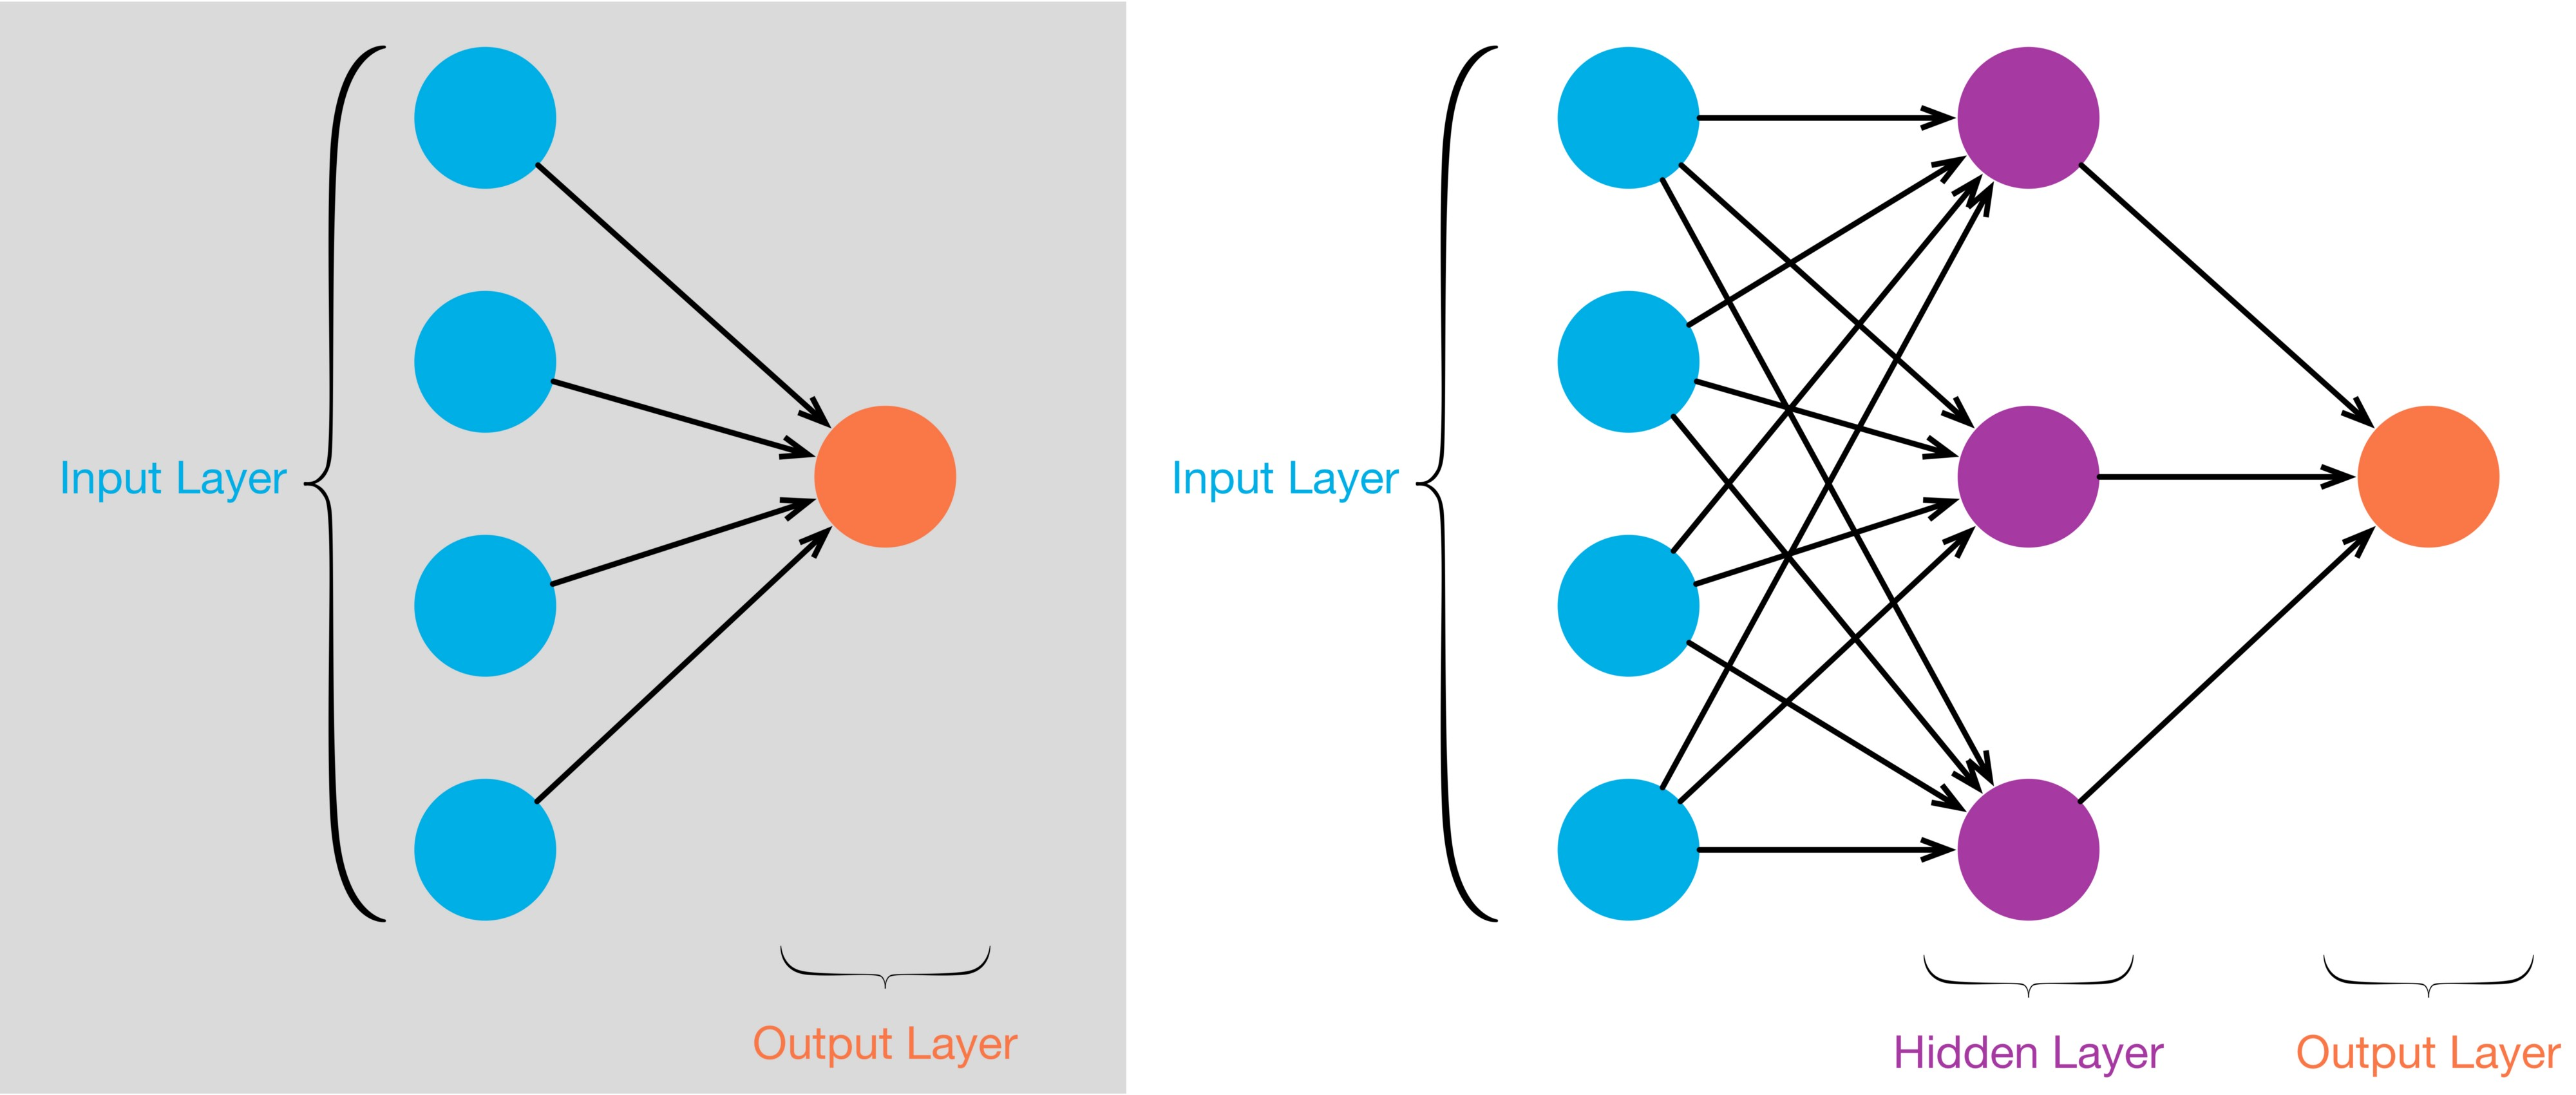
\includegraphics[scale=0.09]{img/nn-layers.jpeg}
\end{center}

Note that the input layer is usually ignored when counting the layers. \\

To understand deeply the 1-layer I strongly recommend Andrew Ng's tutorial for more details or this \href{https://towardsdatascience.com/everything-you-need-to-know-about-neural-networks-and-backpropagation-machine-learning-made-easy-e5285bc2be3a}{article} for a wrap up. \\

Let's now go into deeper details on the working on a 2-layer network.

\section{2-layer NN}

There are already an elephantic number of articles on the maths behind neural networks, so I won't go into much details but rather focus on the points that are, in my view, the most important. \\

For the sake of simplicity, we will use a binary classification. Thus, the labels belong to ($\{0,1\}$). The cost function is:

$$\mathcal{L}(y, \widehat{y})=-[y\log(\widehat{y})+(1-y)\log(1-\widehat{y})]$$

We notice that the loss function decreases when $y \neq \widehat y$, which is expected as we want to penalize wrong classification.

The forward propagation allows to compute the loss functions based on the weights:

\begin{center}
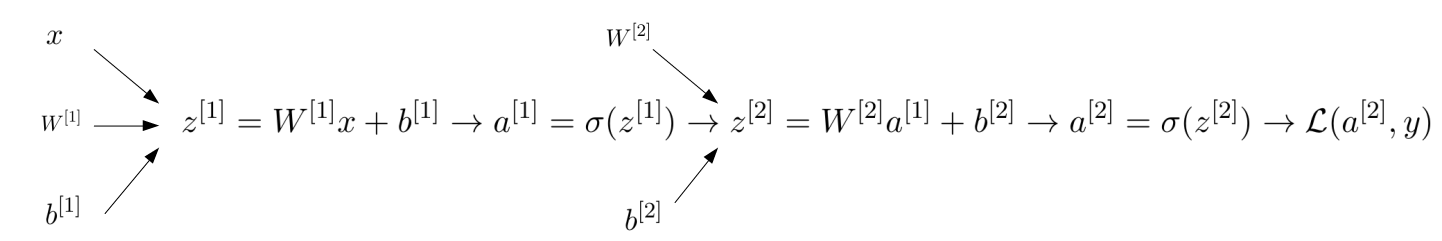
\includegraphics[scale=0.3]{img/NN_2.png}
\end{center}

As we can see here, we use two sets of weights and biases: $W^{[1]}$, $b^{[1]}$, $W^{[2]}$ and $b^{[2]}$. \\

Then, the backward propagation allows to find how to update the weights in order to minimize the loss:

\begin{center}
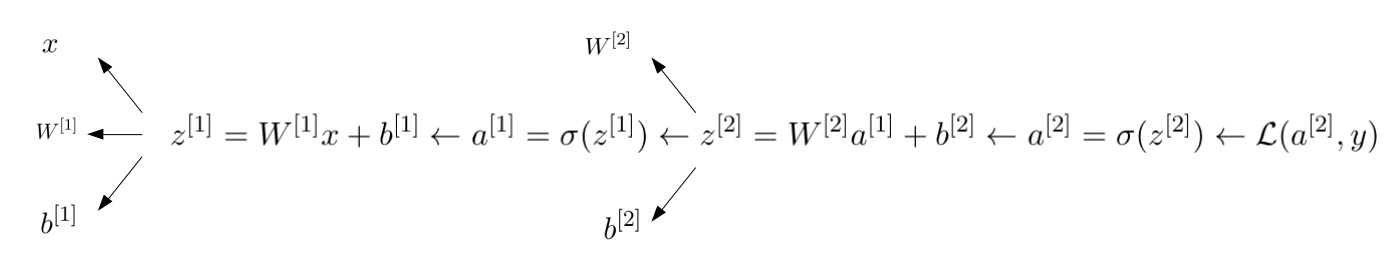
\includegraphics[scale=0.3]{img/NN_2_backward.png}
\end{center}


For the full details on the derivative computation, I explain everything on \href{https://savoga.github.io/machinelearning/neural-network/}{my website} (hopefully I didn't do too many mistakes).

\section{Building the app}

The app will allow the user to provide two types of input: \\

- the shape of the data: blobs, circles or moons \\

- the number of hidden units in the neural network \\

Of course, this is just an example of what types of interactions you can have between the user and the neural network. But as explained in the conclusion of the article, you can add much more parameters! \\

The graphical interfact chosen for the playground is plotly-dash. I am personnaly a big fan of this framework as the \href{https://dash.plotly.com/}{documentation} is quite complete and the \href{https://community.plotly.com/c/dash/16}{community} very active. \\

When developing an app, it is a good practice to separate the modelling part from the graphical part. We will also create a specific module to generate the data. In the end there are 3 python scripts in this app: \\

- utils.py: in this module we simulate data based on the user's preferences \\

- model.py: here we implement the neural network itself! \\

- app.py: everything about the graphical part (buttons, titles etc.) fall in this script \\

\subsection{utils.py}

We will allow the user to choose between three types of data shape: blobs, circles and moons. \\

IMAGE  \\

\subsection{model.py}

In this module we build the neural network logic. As mentioned earlier, we want to build it from scratch so that we understand everything what is happening. 

The tricky part here is to be consistent with the dimensions, especially during the derivative computation:

\lstset{language=Python}
\lstset{frame=lines}
\lstset{caption={Backward propagation}}
\lstset{label={lst:code_direct}}
\lstset{basicstyle=\footnotesize}
\begin{lstlisting}

dz2 = a2-y_train
dw2 = (1/n_samples)*np.dot(dz2,a1.T)
db2 = (1/n_samples)*np.sum(dz2)
dz1 = np.multiply(np.dot(self.weights_2.T,dz2),1-np.power(a1,2))
dw1 = (1/n_samples)*np.dot(dz1,X_train.T)
db1 = (1/n_samples)*np.sum(dz1, axis = 1, keepdims = True)

\end{lstlisting}

 I tried to draw a little schema with the right dimensions: \\

\section{Deployment}

The deployment is done via \href{https://www.heroku.com/}{Heroku}. The clear steps for deployment are explained \href{https://dash.plotly.com/deployment}{here}. As mentioned in the link, "Heroku is one of the easiest platforms for deploying and managing public Flask applications.".

To sum up, the deployment consists in hosting the code in a Github repo, then deploying through Heroku with this command:

\lstset{language=bash}
\lstset{frame=lines}
\lstset{caption={Deploy the app}}
\lstset{label={lst:code_direct}}
\lstset{basicstyle=\footnotesize}
\begin{lstlisting}

$ git push heroku master

\end{lstlisting}

\vspace{5mm}

\section{Key insights}

When playing with the app we can already draw some interesting insights:

- 1 hidden unit gives a linear separation that is especially visible when selecting circles. \\

IMAGE \\

- 2 hidden units give a better separation \\

IMAGE \\

- 3 hidden units give a perfect separation of the clusters when choosing moons.

This illustrates the power of neural networks :) You can think of how good they can be when identifying human faces or finger prints!

\section{Extensions}

The extension possibilities are endless! You can think about adding checkboxes/buttons so that the user can: \\

- the noise (standard deviation) associated with the data generation

- the number of data points to be generated

- the learning rate to be used during the parameter update

- the number of layers \\

For the last point however, I believe it would require significantly more work, especially if you don't use any neural network library (like tensorflow or pytorch) as we do here. \\

Have fun!

\section{Conclusion}

This is my first article on Medium, I'd be happy to get your feedback with a clap and/or a comment. \\